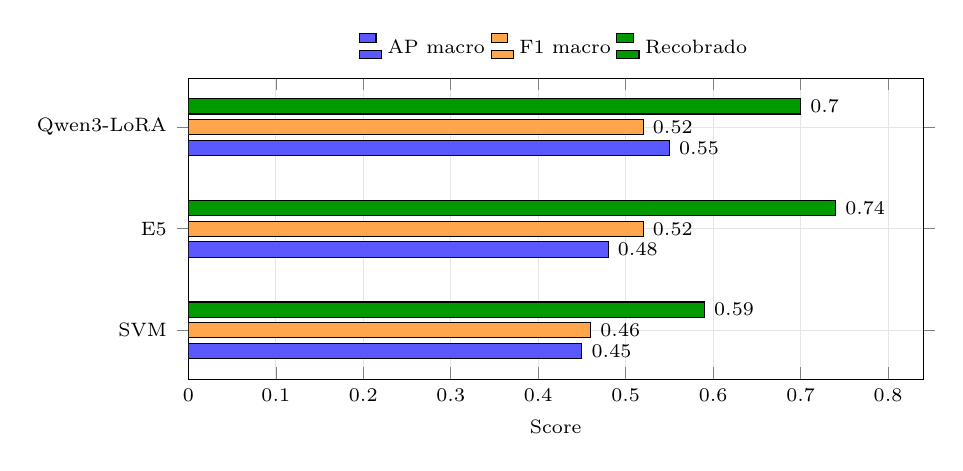
\begin{tikzpicture}
\begin{axis}[
  xbar,
  width=.90\columnwidth,
  height=54mm,
  xmin=0,xmax=.84,
  xlabel={Score},
  symbolic y coords={SVM,E5,Qwen3-LoRA},
  ytick=data,
  bar width=5.5pt,
  enlarge y limits=.24,
  legend style={at={(0.5,1.03)},anchor=south,legend columns=3,font=\scriptsize,draw=none},
  tick label style={font=\scriptsize},
  label style={font=\scriptsize},
  nodes near coords,
  nodes near coords align={horizontal},
  every node near coord/.append style={font=\scriptsize,anchor=west},
  /pgf/number format/fixed,
  /pgf/number format/precision=2,
  grid=major,
  grid style={gray!20}
]
\addplot[fill=blue!65] coordinates {(.45,SVM) (.48,E5) (.55,Qwen3-LoRA)};
\addplot[fill=orange!70] coordinates {(.46,SVM) (.52,E5) (.52,Qwen3-LoRA)};
\addplot[fill=green!60!black] coordinates {(.59,SVM) (.74,E5) (.70,Qwen3-LoRA)};
\legend{AP macro,F1 macro,Recobrado}
\end{axis}
\end{tikzpicture}
